\chapter{Evaluation}
For the evaluation of the tool, I used the CSV files to analyze the quantitative data produced by the tool. To assess whether the roads generated by ChatGPT align with the description and whether ChatGPT generates diverse roads with the same prompt, I conducted a user study. The results of the data analysis will be described below.

\section{Analysis of the CSV Files}
To analyze generation statistics, three prompts of varying specificity were used: "a road", "an uphill road with 3 turns", and "a road going uphill for 2 turns, followed by a straight downhill segment, ending in a left turn". A combined total of 300 roads were generated, with 100 roads produced for each prompt. Following the simulations, two CSV files were created for each prompt. One contained generation statistics (number of roads generated, valid/invalid counts), while the other recorded instances of cars driving out of their lanes. Of the 300 roads generated, 182 successfully passed validation, with 118 failing. Among the 182 roads simulated, the car steered out of its lane in 8 instances.

Among the 100 roads generated using the prompt "a road," 88 successfully passed validation, and 1 of those 88 roads resulted in the car driving out of the lane. For the prompt "an uphill road with 3 turns," out of the 100 roads generated, 57 met validation criteria, with 2 of those 57 ending with the car steering out of the lane. Lastly, from the 100 roads generated with the prompt "a road going uphill for 2 turns, followed by a straight downhill segment, ending in a left turn," only 37 successfully passed validation, with 5 out of those 37 roads ending with the car driving out of the lane.

This indicates that when prompts are more generic and the language model has more freedom, it tends to better adhere to the specified rules, such as the map size. However, roads generated from more general prompts seem to place less emphasis on testing the lane-keeping functionality of the self-driving agent compared to roads generated from more specific prompts.

The chi-squared test was used to determine the statistical significance of these results. Regarding the number of valid roads generated per prompt, the hypotheses were as follows:

H0: the prompt does not influence the number of valid roads generated
H1: the prompt does influence the number of valid roads generated

An alpha value of 0.05 was chosen.

First, a contingency table (\ref{contingency_validity}) was created to display the counts of valid and invalid roads generated for each prompt. This table was then used to derive the expected values table (\ref{expected_values_validity}), calculated using the formula \(\frac{row\ total * column\ total}{grand\ total}\) for each cell. With these two tables, the chi-square score was computed by applying the formula \(\frac{(observed\ value - calculated\ value)^2}{calculated\ value}\) to each element and summing the results \ref{chi_sq_validity}.

The degrees of freedom are determined by the formula \((number\ of\ rows - 1) * (number\ of\ columns - 1)\). The critical chi-square value can be found in the chi-square distribution table in Appendix \ref{chisq_dist_table}, using the degrees of freedom and the alpha value. Since the calculated chi-square value is 55.35, the critical chi-square value is 5.99, and 55.35 is greater than 5.99, the null hypothesis H0 is rejected. This indicates that the prompt does influence the number of valid roads generated.

In the following tables, the prompt "a road" is referred to as prompt 1, the prompt "an uphill road with 3 turns" is referred to as prompt 2, and the prompt "a road going uphill for 2 turns, followed by a straight downhill segment, ending in a left turn" is referred to as prompt 3.


\begin{table}[H]
    \centering
    \begin{tabular}{|c|c|c|c|} \hline 
         &  valid&  invalid& total\\ \hline 
         prompt 1&  88&  12& 100\\ \hline 
         prompt 2&  57&  43& 100\\ \hline 
         prompt 3&  37&  63& 100\\ \hline 
         total&  182&  118& 300\\ \hline
    \end{tabular}
    \caption{Road Validity Contingency Table}
    \label{contingency_validity}
\end{table}

\begin{table}[H]
    \centering
    \begin{tabular}{|c|c|c|c|} \hline 
         &  valid&  invalid& total\\ \hline 
         prompt 1&  60.67&  39.33& 100\\ \hline 
         prompt 2&  60.67&  39.33& 100\\ \hline 
         prompt 3&  60.67&  39.33& 100\\ \hline 
         total&  182&  118& 300\\ \hline
    \end{tabular}
    \caption{Road Validity Expected Values Table}
    \label{expected_values_validity}
\end{table}

\begin{table}[H]
    \centering
    \begin{tabular}{|c|c|c|c|} \hline 
         &  observed&  calculated& \(\frac{(o-c)^2}{c}\) \\ \hline 
         &  88&  60.67& 12.32\\ \hline 
         &  57&  60.67& 0.22\\ \hline 
         &  37&  60.67& 9.32\\ \hline 
         &  12&  39.33& 18.99\\ \hline 
         &  43&  39.33& 0.34\\ \hline 
         &  63&  39.33& 14.24\\ \hline 
         total&  &  & 55.35\\ \hline
    \end{tabular}
    \caption{Road Validity Chi-Square Calculation}
    \label{chi_sq_validity}
\end{table}

\section{Survey}
For the user study, I distributed a survey to 11 individuals engaged in research or work related to autonomous vehicles. Of these, ten respondents provided answers.

\subsection{Survey structure}
The survey was split into three main sections. The first section aimed to gather demographic information from the participants. The second section asked participants to rate the alignment between a road and the prompt it was generated with. To assist in their evaluation, participants were provided with a bird's-eye view plot, an altitude plot, and two videos depicting a car driving on the road. The first video displayed the car from a third-person perspective, while the second one provided a view from the car's bonnet. In the final section, participants were asked to rate the similarity between two roads generated using the same prompt. For this task, the participants were provided with the altitude plot and the bird's eye view of each road stacked on top of each other, alongside two videos featuring a split-screen view of a car driving on both roads simultaneously. The first split-screen video showed the two cars from a third-person view, while the second one provided a view from the car's bonnets.

Given that all roads used in the user study fall within the coordinate range of 0 to 220, the axes of the bird's-eye view plot are set to span from point 0 to 220, with each unit on the plot representing 1 meter. The axis dimensions were selected to offer a neutral perspective of the roads, avoiding any emphasis on the turns of one road over another. Given that the maximum altitude and longest road length are restricted to 20 and 200 meters, respectively, these factors determine the scaling of the axes for visualizing distance and height in the plot.

\subsection{Survey results}
In this section, I will describe the results of the survey by section.
\subsubsection{Demographic Data}
The participants were asked about their age, occupation, possession of a driver's license, number of countries they have driven in, prior experience with generative AI, and familiarity with driving simulators.

Four participants fall within the age range of 20 to 29 years, five are aged between 30 to 39, and one participant is aged between 40 to 49 (see Figure \ref{age}). Nine participants hold a driver's license, while one does not (see Figure \ref{drivers-license}). Each participant has driven in at least one country (see Figure \ref{countries-driven-in}). Seven participants use generative AI regularly, while three reported using it occasionally (see Figure \ref{genai}). Eight participants use driving simulators regularly, one uses them occasionally, and one participant has never used a driving simulator before (see Figure \ref{driving-simulator}).

\begin{figure}[H]
    \centering
    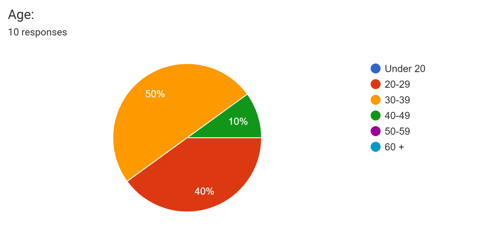
\includegraphics[width=0.6\linewidth]{images/age.png}
    \caption{Age}
    \label{age}
\end{figure}

\begin{figure}[H]
    \centering
    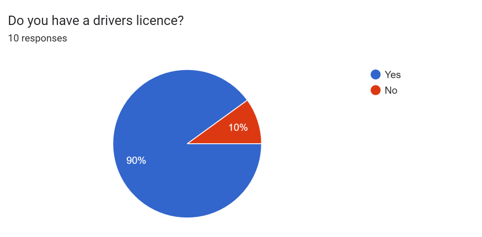
\includegraphics[width=0.5\linewidth]{images/drivers_license.png}
    \caption{Driver's license}
    \label{drivers-license}
\end{figure}

\begin{figure}[H]
    \centering
    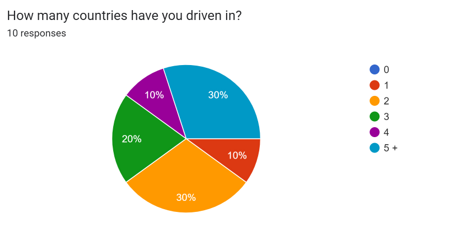
\includegraphics[width=0.6\linewidth]{images/countries_driven_in.png}
    \caption{Countries driven in}
    \label{countries-driven-in}
\end{figure}

\begin{figure}[H]
    \centering
    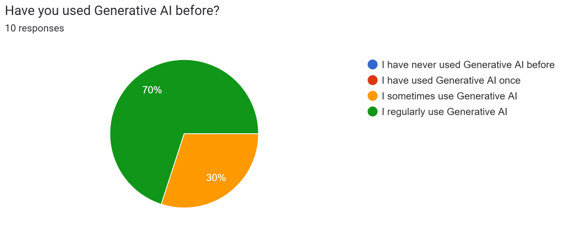
\includegraphics[width=0.7\linewidth]{images/gen_ai.png}
    \caption{Generative AI}
    \label{genai}
\end{figure}

\begin{figure}[H]
    \centering
    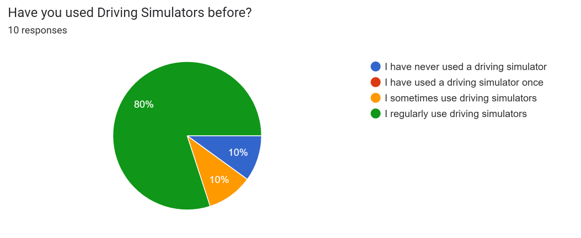
\includegraphics[width=0.7\linewidth]{images/driving_sim.png}
    \caption{Driving Simulator}
    \label{driving-simulator}
\end{figure}

\subsubsection{Road-Prompt Alignment}
In the section concerning Road-Prompt Alignment, participants are tasked with assessing how well a given road corresponds to a provided prompt. This evaluation involves two main components: the overall suitability of the road and its adherence to specific criteria, such as the number of turns, incline, and sequence/order of turns. For visual reference, the participants were presented with an image showing the road plot from both a bird's-eye view and one illustrating altitude side by side as depicted in Figure \ref{road_vis}. Additionally, users had access to two videos: one featuring a car driving on the road from a third-person perspective (see Figure \ref{third-person-view}) and another showing the view from a camera mounted on the car's bonnet (see Figure \ref{bonnet-view}).

\begin{figure}[H]
    \centering
    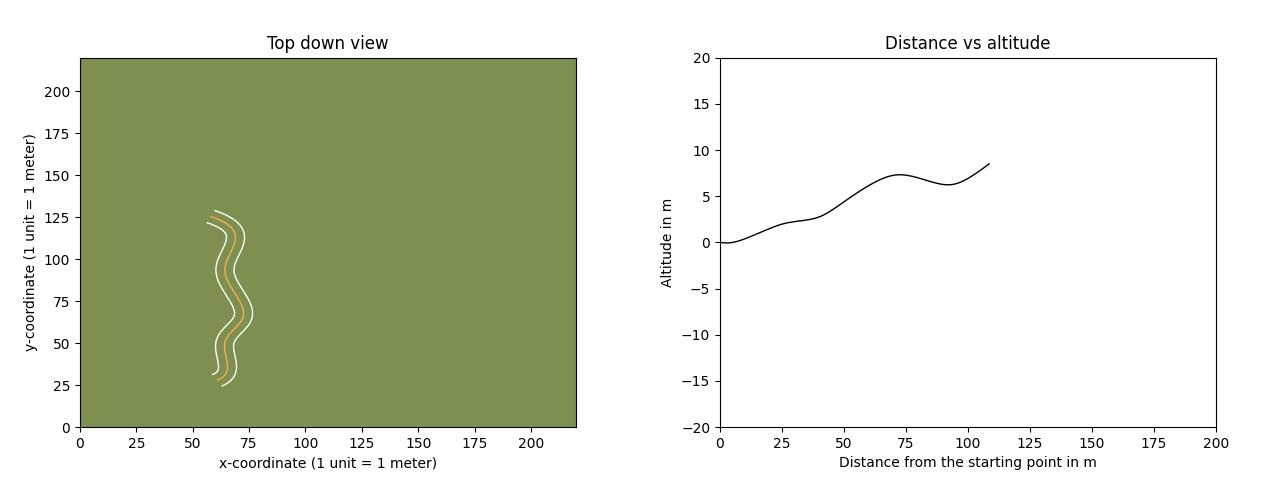
\includegraphics[width=1\linewidth]{images/road3.jpg}
    \caption{Visualization of a road generated with the prompt "a serpentine road"}
    \label{road_vis}
\end{figure}

\begin{figure}[H]
    \centering
    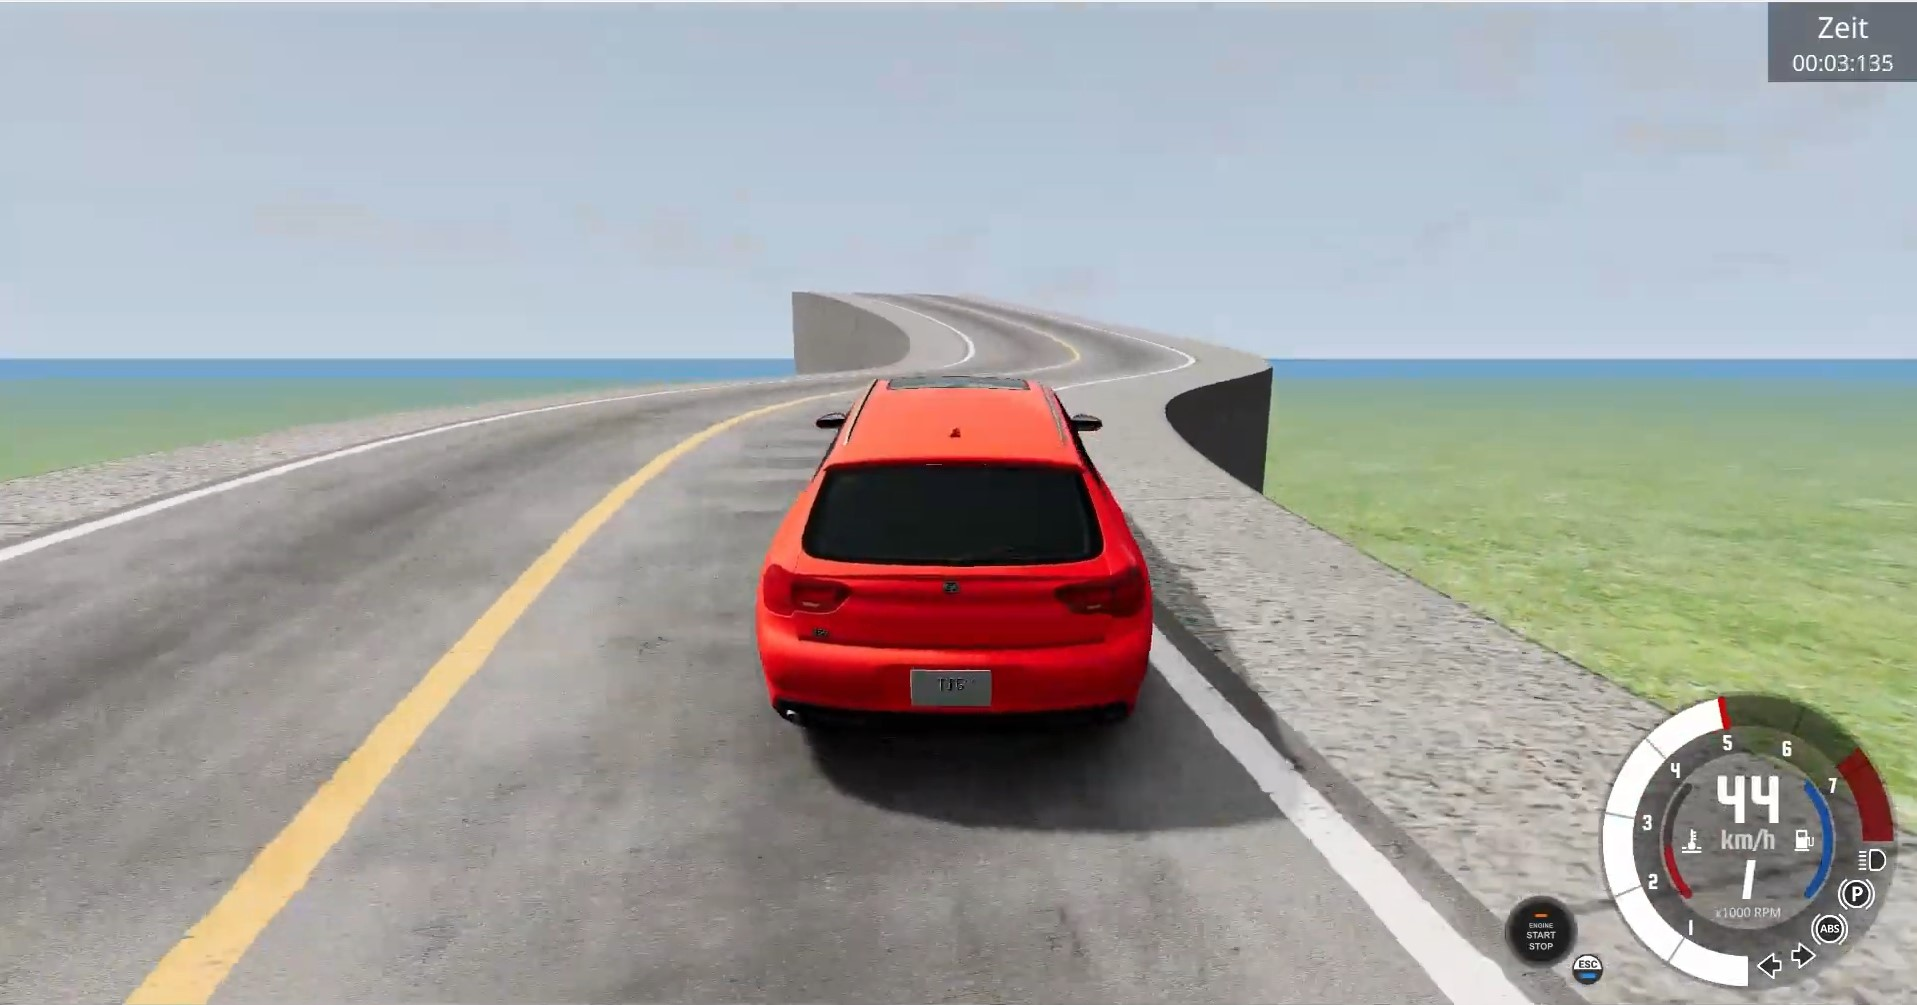
\includegraphics[width=0.5\linewidth]{images/Third_Person_View.jpg}
    \caption{Screenshot from a Video with a Third Person Perspective of a car driving on the road}
    \label{third-person-view}
\end{figure}

\begin{figure}[H]
    \centering
    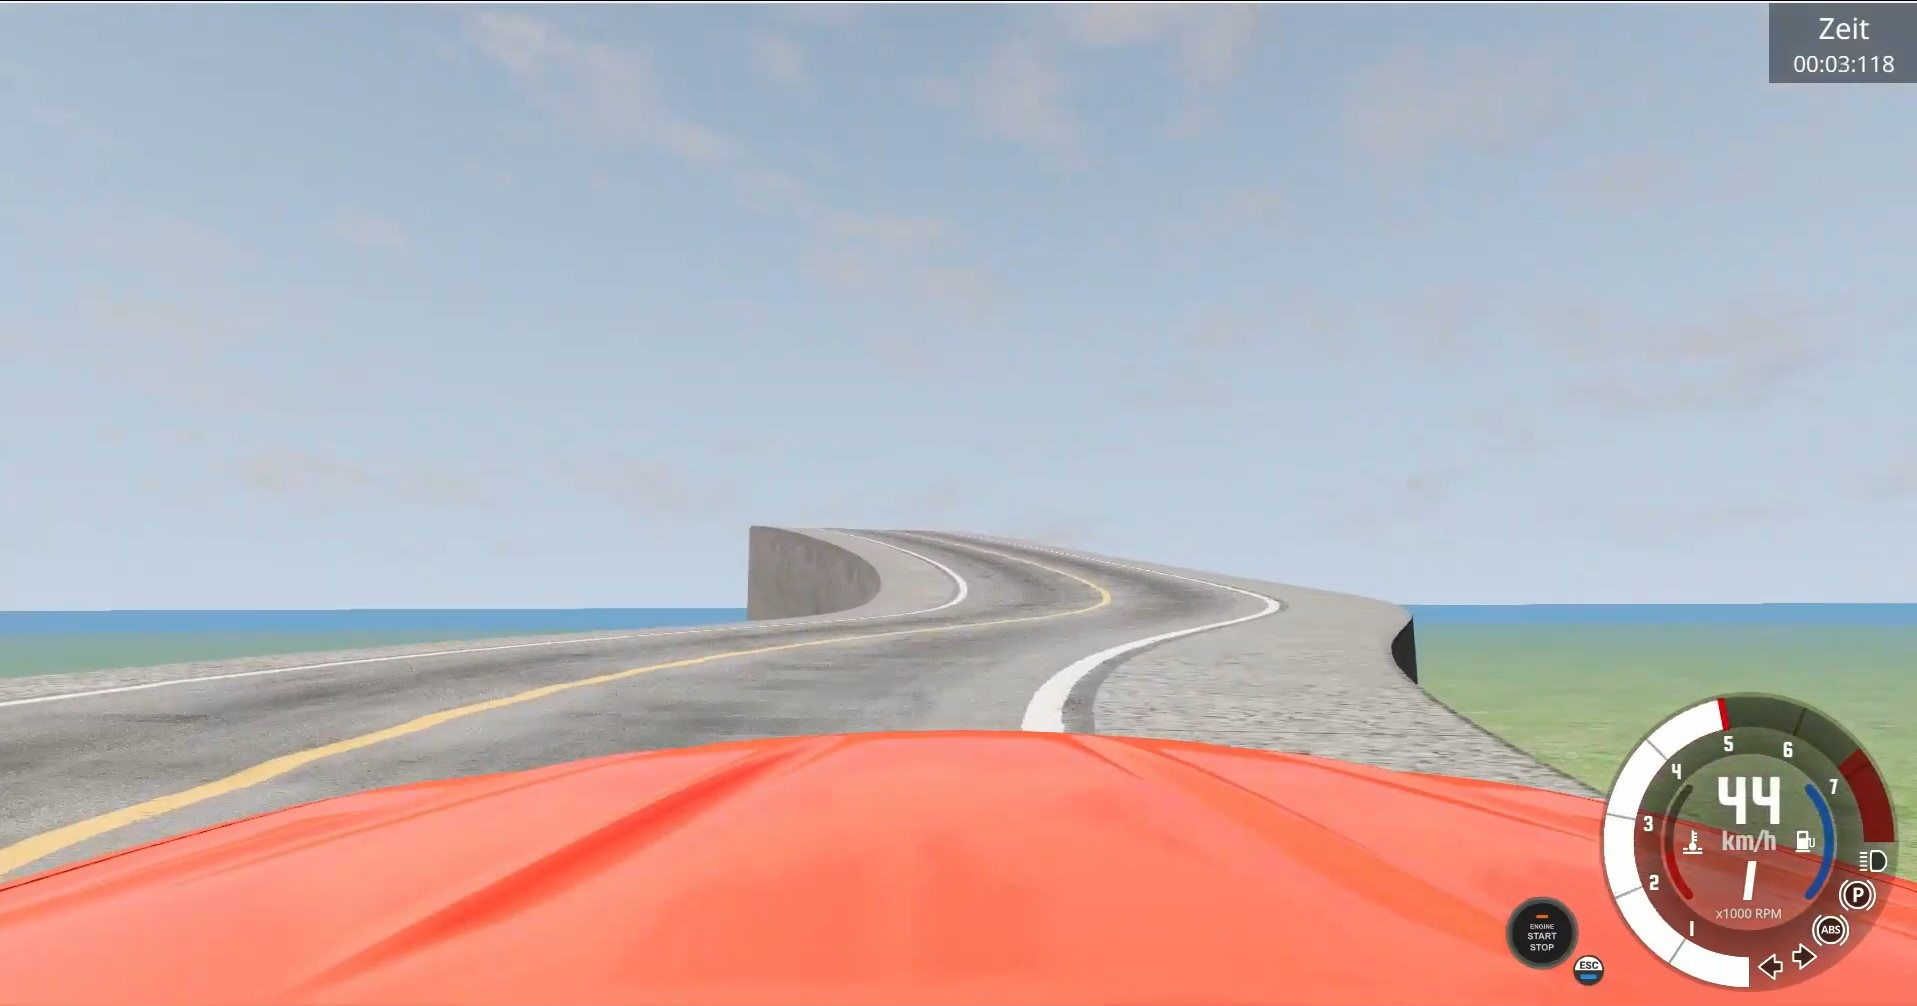
\includegraphics[width=0.5\linewidth]{images/Bonnet_Perspective.jpg}
    \caption{Screenshot from a Video with a Bonnet Perspective of a car driving on the road}
    \label{bonnet-view}
\end{figure}


Four prompts were used for road creation: "a serpentine road", "an uphill road with 3 turns", "a road going uphill for 3 turns and downhill for 2 turns", and "a road going uphill for 2 turns, followed by a straight downhill segment, ending with a left turn." These prompts were chosen to transition from general to more specific. The participants evaluated how well the visualized road matched the respective prompt in both overall fit and specific criteria. Additionally, participants were given the option to provide extra feedback for each road. The participants were required to select from the options "does not match the description at all", "generally does not match the description", "somewhat matches the description", "mostly matches the description", and "perfectly matches the description" in order to cast their votes.

The prompt "a serpentine road" was the most generic prompt used for road generation (see figure \ref{road_vis}). Therefore, participants were only required to rate their overall fit with the prompt. As depicted in figure \ref{serpentine_alignment}, while one participant disagreed, the majority agreed that the road aligned well. Five out of ten participants rated it as a perfect match, one as mostly matching, and three as somewhat matching.

\begin{figure}[H]
    \centering
    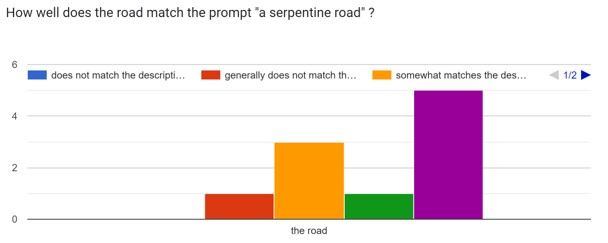
\includegraphics[width=0.75\linewidth]{images/serpentine_general.jpg}
    \caption{Results of the general road-prompt alignment for "a serpentine road"}
    \label{serpentine_alignment}
\end{figure}


The second prompt used was "an uphill road with 3 turns" (see figure \ref{u3t-vis}), which was more detailed as it specified both the incline and the number of turns. Participants indicated that the road generally aligned with the prompt (see figure \ref{u3t-general-alignment}). Regarding the incline, the majority voted that it perfectly matched the prompt, while opinions were divided on the number of turns, with more participants indicating somewhat or mostly matching (see figure \ref{u3t-specific-alignment}). Multiple respondents provided additional feedback, noting a turn starting at the road's end.

\begin{figure}[H]
    \centering
    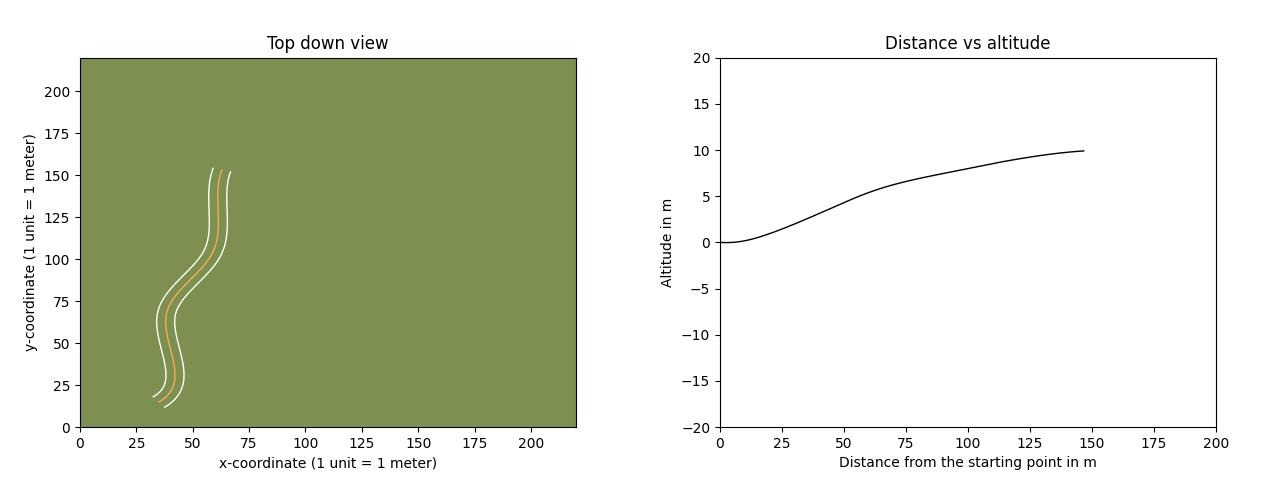
\includegraphics[width=0.75\linewidth]{images/road1.jpg}
    \caption{Visualization of a road generated with the prompt "an uphill road with 3 turns"}
    \label{u3t-vis}
\end{figure}

\begin{figure}[H]
    \centering
    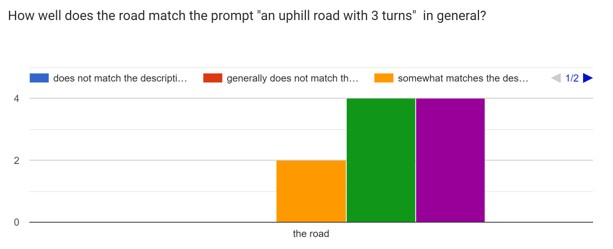
\includegraphics[width=0.75\linewidth]{images/u3t_general.jpg}
    \caption{Results of the general road-prompt alignment for "an uphill road with 3 turns"}
    \label{u3t-general-alignment}
\end{figure}

\begin{figure}[H]
    \centering
    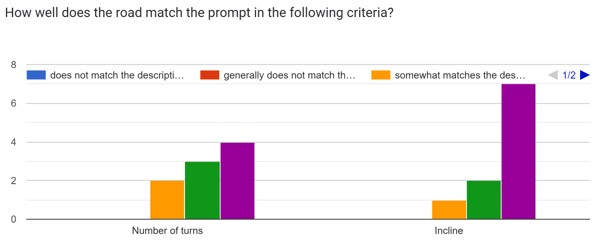
\includegraphics[width=0.75\linewidth]{images/u3t_criteria.jpg}
    \caption{Results of the road-prompt alignment in specific criteria for "an uphill road with 3 turns"}
    \label{u3t-specific-alignment}
\end{figure}

The prompt "a road going uphill for 3 turns and downhill for 2 turns" (see figure \ref{u3t-d2t-vis}) introduced an additional level of specificity by incorporating changes in incline. Although participants generally agreed that the road aligned with the prompt (see figure \ref{u3t-d2t-general}, closer inspection of specific aspects revealed mismatches. While the incline and the number of uphill turns closely matched the prompt, the count of downhill turns did not (figure \ref{u3t-d2t-specific}). In the additional feedback, several participants highlighted the absence of a downhill turn. One participant noted that while the LLM interprets the incline correctly, "counting" the turns does not seem to be a task that it performs well in.

\begin{figure}[H]
    \centering
    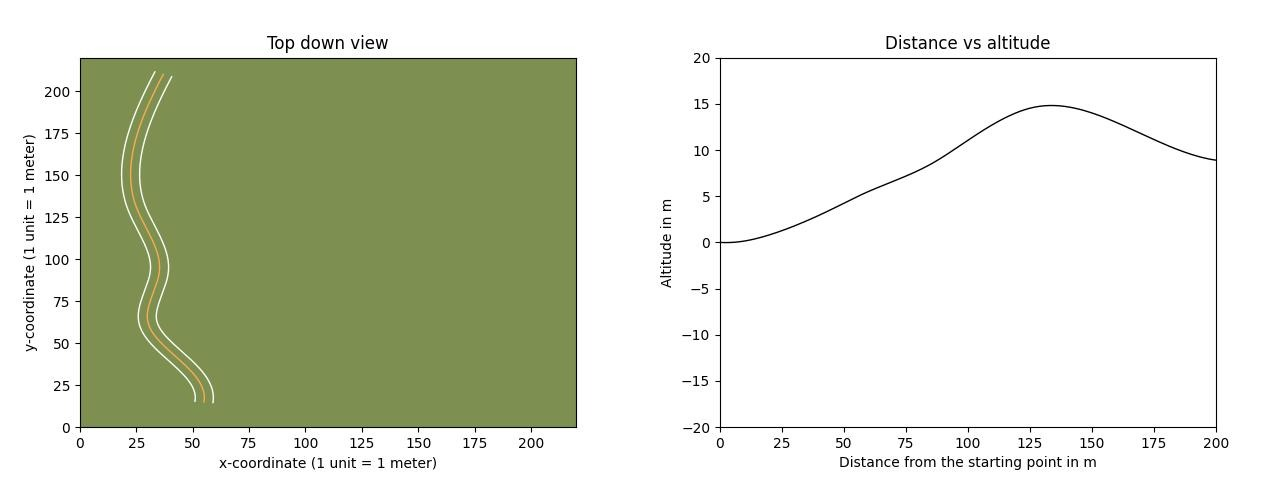
\includegraphics[width=0.75\linewidth]{images/u3t_d2t_vis.jpg}
    \caption{Visualization of a road generated with the prompt "a road going uphill for 3 turns and downhill for 2 turns"}
    \label{u3t-d2t-vis}
\end{figure}

\begin{figure}[H]
    \centering
    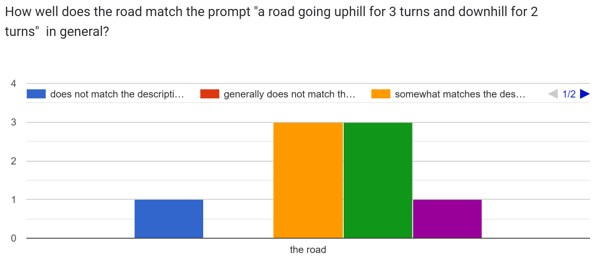
\includegraphics[width=0.75\linewidth]{images/u3t_d2t_general.jpg}
    \caption{Results of the general road-prompt alignment for "a road going uphill for 3 turns and downhill for 2 turns"}
    \label{u3t-d2t-general}
\end{figure}

\begin{figure}[H]
    \centering
    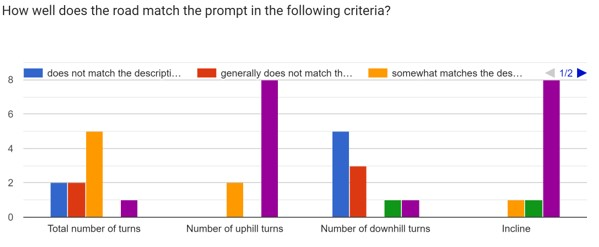
\includegraphics[width=0.75\linewidth]{images/u3t_d2t_specific.jpg}
    \caption{Results of the road-prompt alignment in specific criteria for "a road going uphill for 3 turns and downhill for 2 turns"}
    \label{u3t-d2t-specific}
\end{figure}

The most detailed prompt used is "a road going uphill for 2 turns, followed by a straight downhill segment, ending in a left turn" (figure \ref{most-specific-vis}). The prompt introduces a sequence for the road segments. Although most participants agreed that the road matched the prompt (figure \ref{most-specific-general}), some were unsure about the total number of turns \ref{most-specific-specific-criteria}. In additional comments, two participants mentioned the difficulty in determining whether there was only one turn or two in the uphill segments. Meanwhile, one participant expressed uncertainty about the presence of an additional turn in the uphill segment.

\begin{figure}[H]
    \centering
    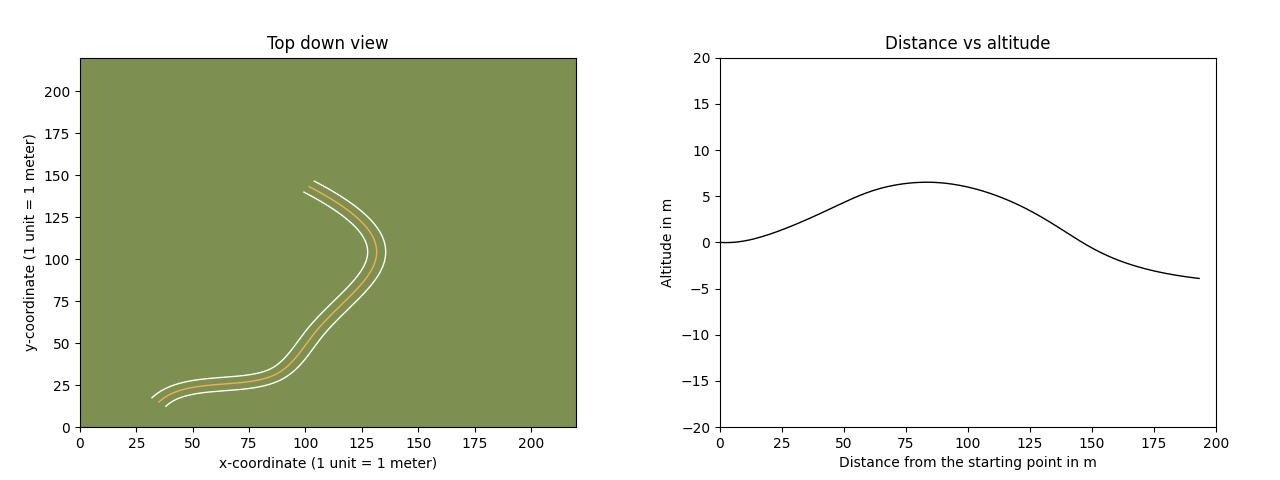
\includegraphics[width=0.75\linewidth]{images/road_height.jpg}
    \caption{Visualization of a road generated with the prompt "a road going uphill for 2 turns, followed by a straight downhill segment, ending in a left turn"}
    \label{most-specific-vis}
\end{figure}

\begin{figure}[H]
    \centering
    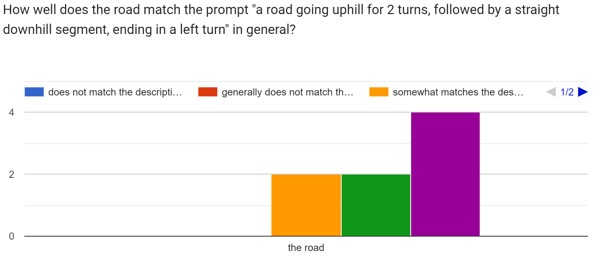
\includegraphics[width=0.75\linewidth]{images/most_specific_general.jpg}
    \caption{Results of the general road-prompt alignment for "a road going uphill for 2 turns, followed by a straight downhill segment, ending in a left turn"}
    \label{most-specific-general}
\end{figure}

\begin{figure}[H]
    \centering
    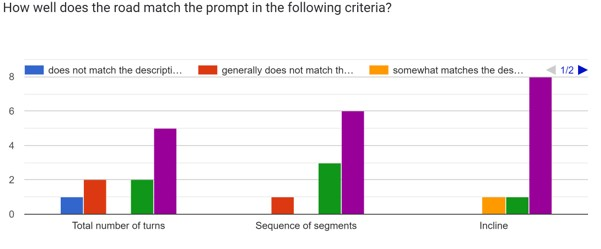
\includegraphics[width=0.75\linewidth]{images/most_specific_specific.jpg}
    \caption{Results of the road-prompt alignment in specific criteria for "a road going uphill for 2 turns, followed by a straight downhill segment, ending in a left turn"}
    \label{most-specific-specific-criteria}
\end{figure}


Reviewing the results, it seems that, as one user pointed out, the LLM performs well at interpreting the incline of the prompts but struggles with accurately identifying the specified number of turns.

\subsubsection{Road Similarity}
In the Road Similarity section, participants were presented with pairs of roads to evaluate their resemblance to each other. Visualizations presented both road plots, one above the other, as shown in figure \ref{comparison_u3t}. Additionally, participants were shown split-screen videos featuring cars driving along both roads simultaneously, with one providing a third-person perspective (figure \ref{splitscreen-tp}) and the other showing the car's perspective from the bonnet (figure \ref{splitscreen-bonnet}). Participants were then prompted to rate the general similarity between the roads and their similarity in specific criteria. Ratings ranged from "definitely different" to "basically the same road" for general similarity and from "definitely different" to "(almost) identical" for specific criteria.

\begin{figure}[H]
    \centering
    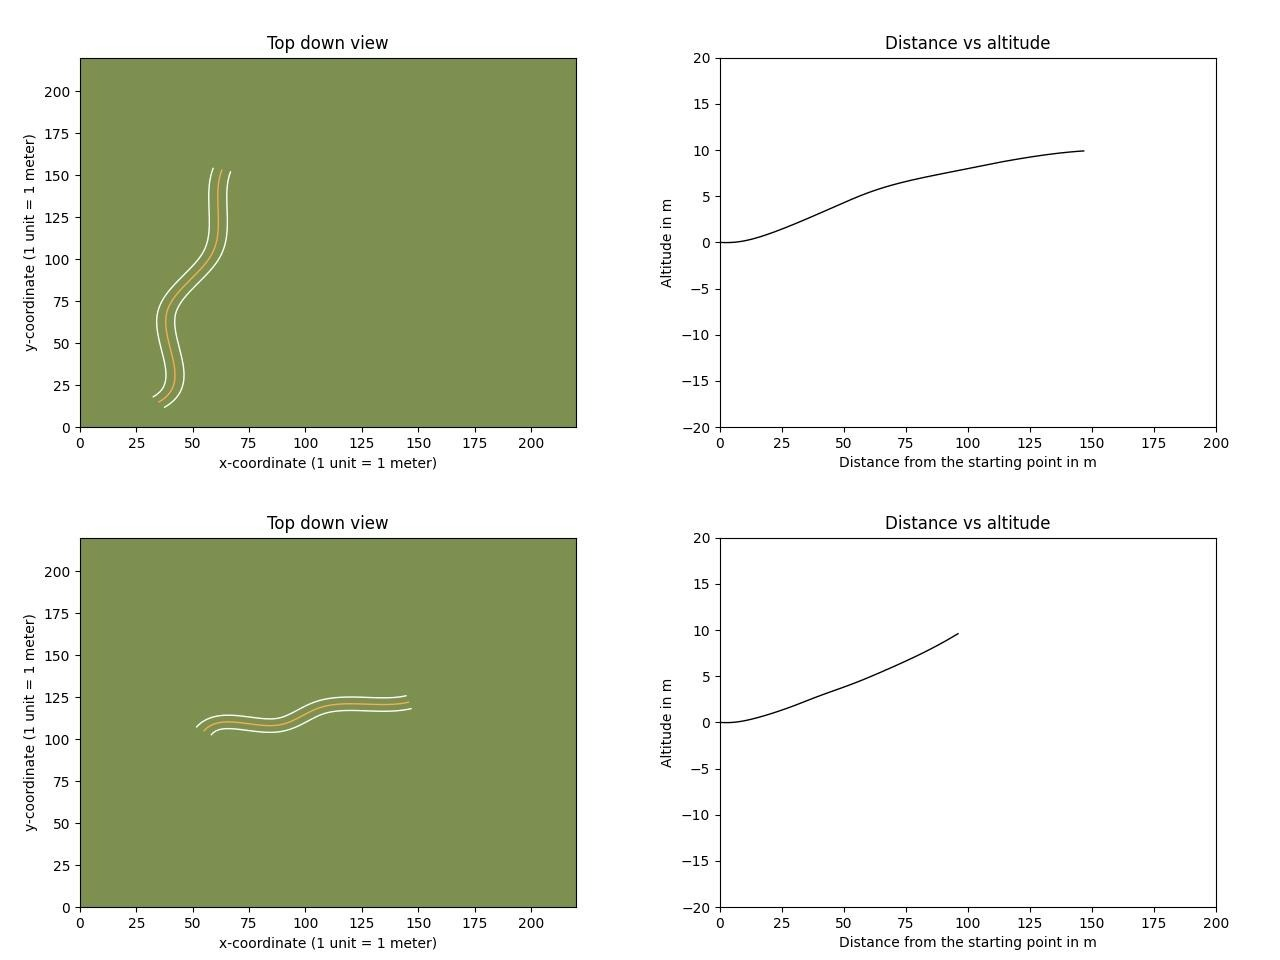
\includegraphics[width=0.75\linewidth]{images/road1_road2.jpg}
    \caption{Comparison of 2 roads generated with the prompt "an uphill road with 3 turns"}
    \label{comparison_u3t}
\end{figure}

\begin{figure}[H]
    \centering
    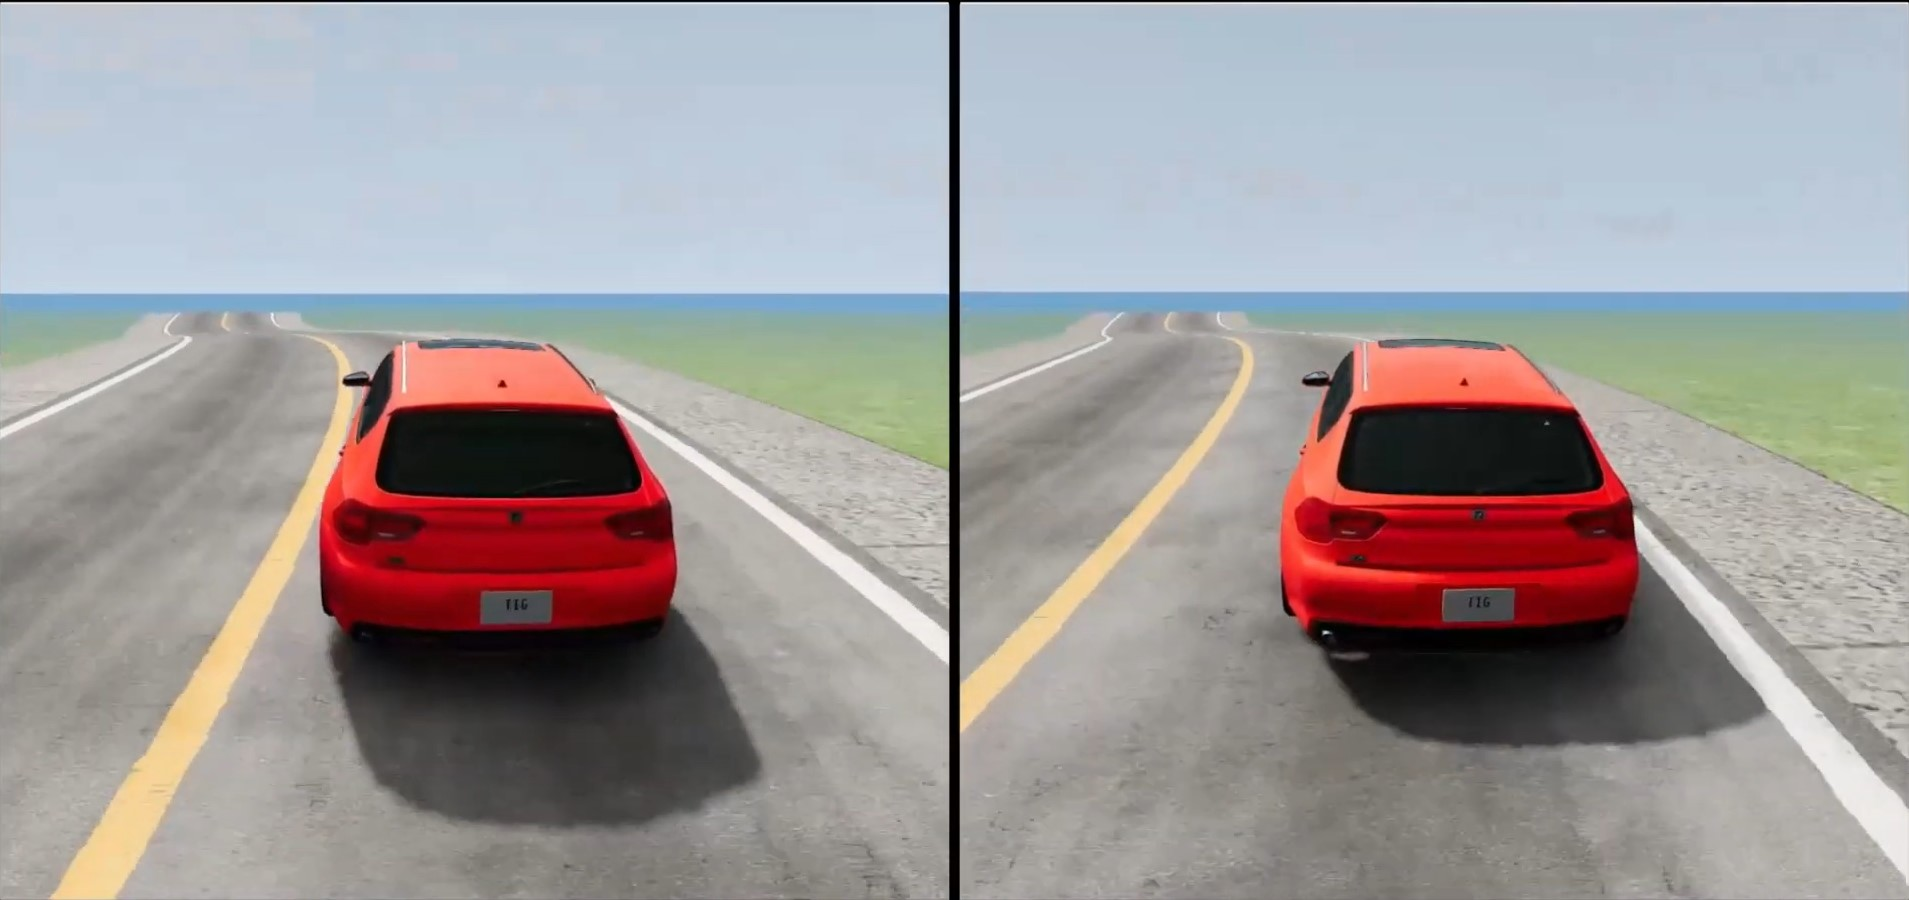
\includegraphics[width=0.75\linewidth]{images/splitscreen_tp_view.jpg}
    \caption{Screenshot from a Split-Screen Video with a Third Person Perspective}
    \label{splitscreen-tp}
\end{figure}

\begin{figure}[H]
    \centering
    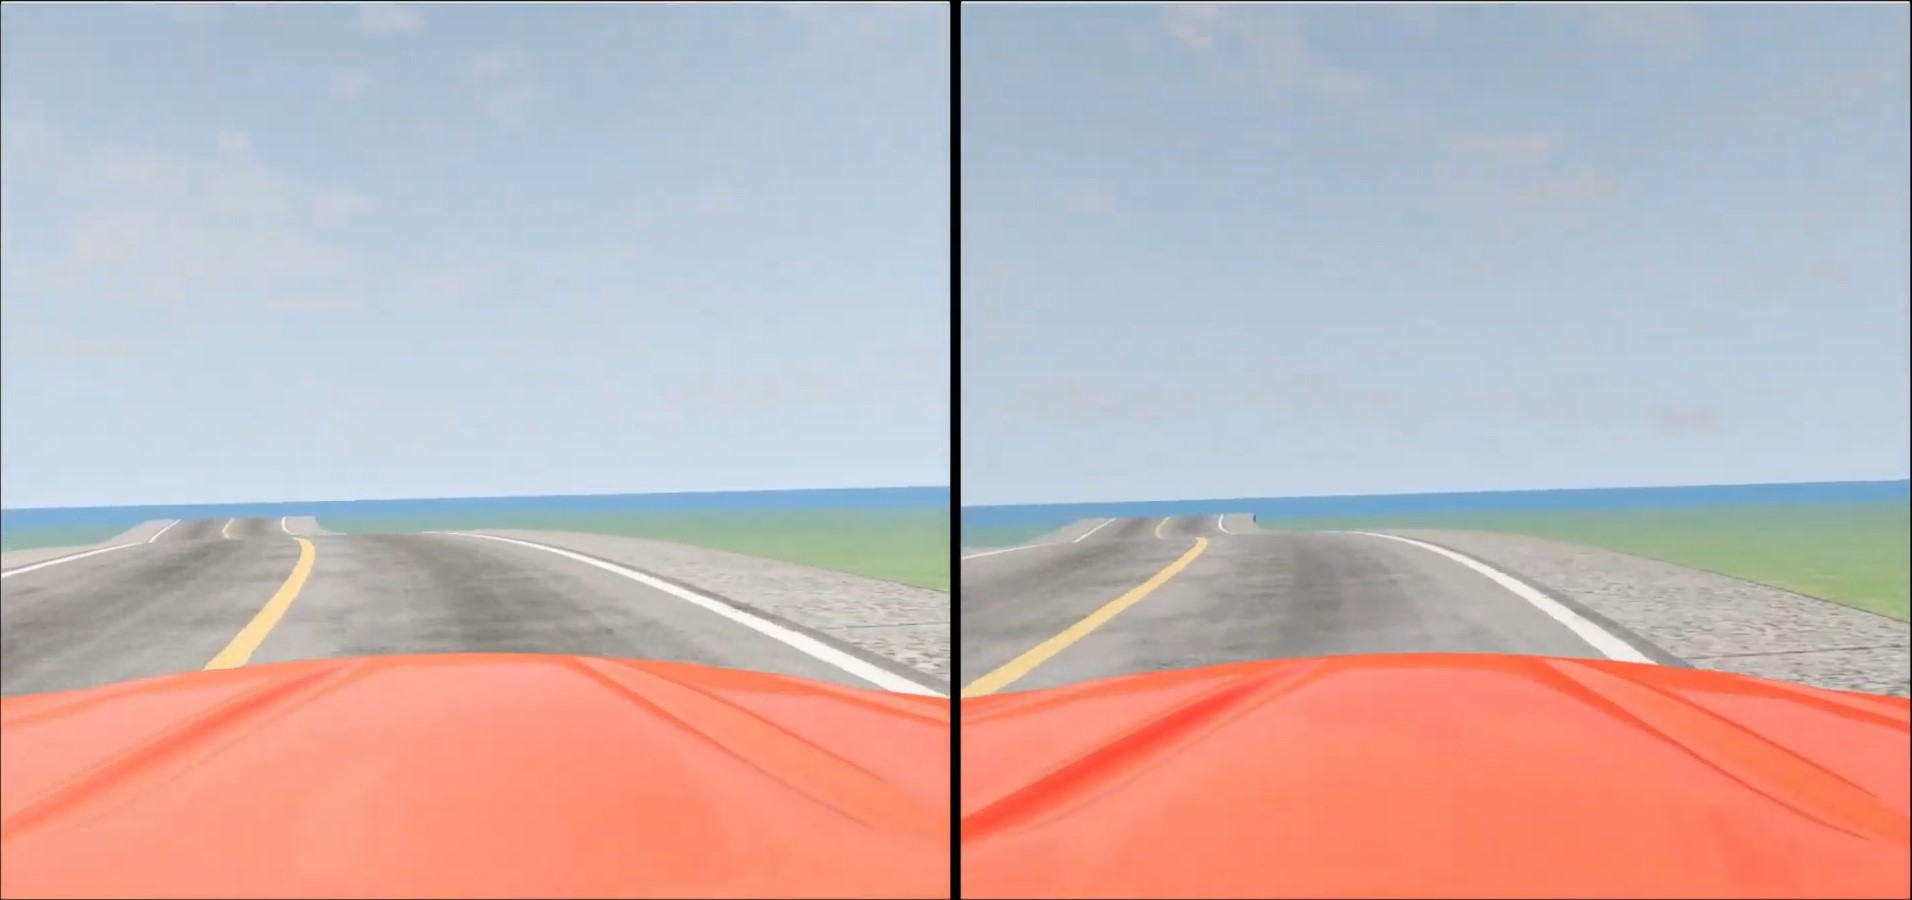
\includegraphics[width=0.75\linewidth]{images/splitscreen_bonnet_view.jpg}
    \caption{Screenshot from a Split-Screen Video with a Bonnet Perspective}
    \label{splitscreen-bonnet}
\end{figure}


The participants generally found the first two roads (figure \ref{comparison_u3t}), which were generated with the prompt "an uphill road with 3 turns",  to be dissimilar, as illustrated in Figure \ref{general_similarity_uphill_road}. Although there was agreement on the similarity in the number of turns, differences were noted in the sequence of turns and the length of the road, which were distinctly perceived as dissimilar. Opinions on the road's incline varied, with three participants rating it as identical while another three rated it as mostly dissimilar (see figure \ref{specific_similarity_uphill_road}).


\begin{figure}[H]
    \centering
    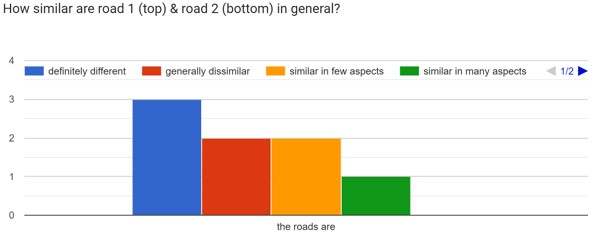
\includegraphics[width=0.75\linewidth]{images/similarity_a_road.jpg}
    \caption{General similarity of the two roads generated with the prompt "an uphill road with 3 turns"}
    \label{general_similarity_uphill_road}
\end{figure}

\begin{figure}[H]
    \centering
    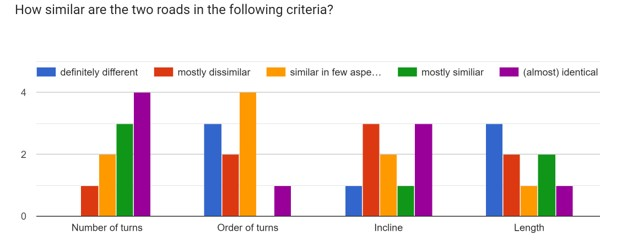
\includegraphics[width=0.75\linewidth]{images/similarity_a_road_specific.jpg}
    \caption{Similarity in certain criteria of the two roads generated with the prompt "an uphill road with 3 turns"}
    \label{specific_similarity_uphill_road}
\end{figure}


The second pair of roads, generated with the prompt "a road" (figure \ref{comparison_a_road}), were perceived as identical (figure \ref{general_similarity_a_road}). Participants rated the roads as identical across all criteria (figure \ref{specific_similarity_a_road}). Several participants noted in the additional comments that the only difference was the orientation of the roads in the bird's eye view plot.


\begin{figure}[H]
    \centering
    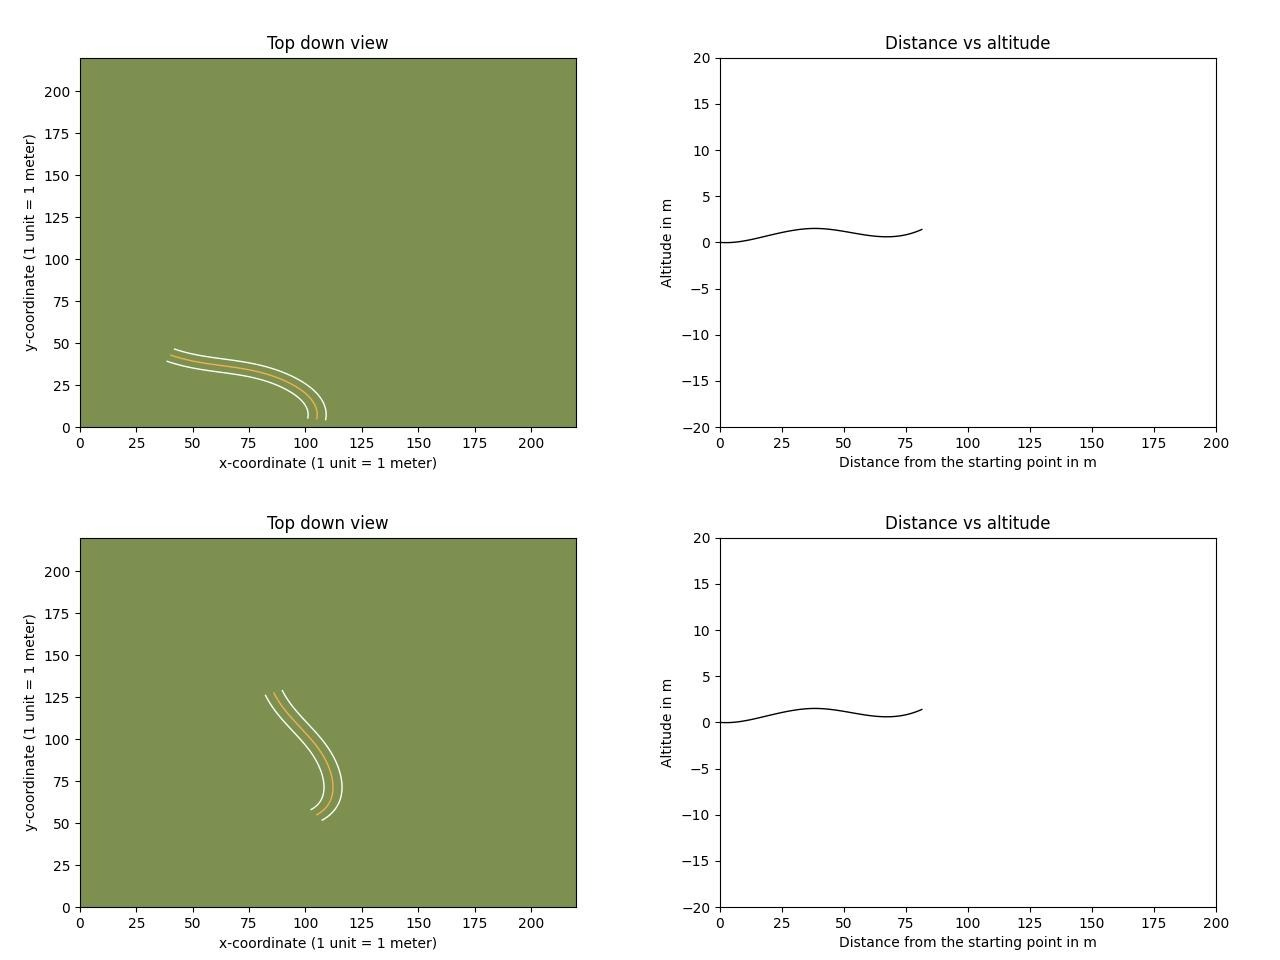
\includegraphics[width=0.75\linewidth]{images/road2_road3.jpg}
    \caption{Comparison of 2 roads generated with the prompt "a road"}
    \label{comparison_a_road}
\end{figure}

\begin{figure}[H]
    \centering
    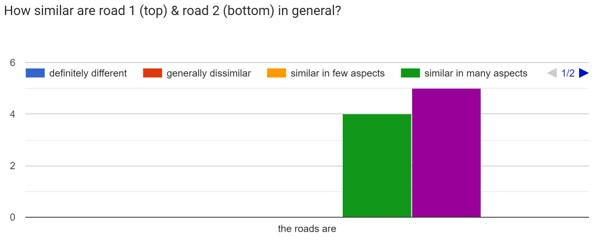
\includegraphics[width=0.75\linewidth]{images/similarity2_general.jpg}
    \caption{General similarity of the two roads generated with the prompt "a road"}
    \label{general_similarity_a_road}
\end{figure}

\begin{figure}[H]
    \centering
    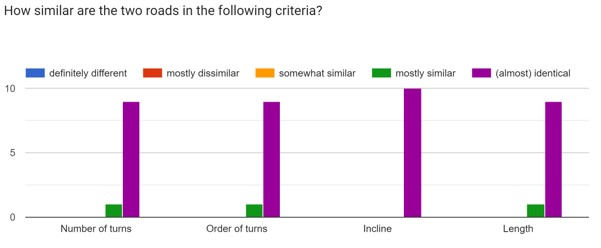
\includegraphics[width=0.75\linewidth]{images/similarity2_specific.jpg}
    \caption{Similarity in certain criteria of the two roads generated with the prompt "a road"}
    \label{specific_similarity_a_road}
\end{figure}

In conclusion, the LLM is proficient in generating roads that meet specific criteria outlined in the prompts. While it accurately interprets inclines, determining the number of turns remains a challenge. When presented with identical prompts, ChatGPT sometimes produces roads that are almost identical, with the main difference being their orientation.


\section{Conclusion}

This section summarizes the results to address the research question \textbf{Can generative AI be used to automatically create three-dimensional roads for testing autonomous vehicles?}

The results imply that Generative AI has the potential to create virtual roads that are appropriate for testing autonomous vehicles. ChatGPT was used due to its accessibility and seamless integration via the OpenAI API. Despite the model not being trained for this particular use case, it produced roads that met most requirements. The user study indicated that while ChatGPT performed well in interpreting road inclines, it struggled with generating the correct number of turns and stressing the lane-keeping functionality of the self-driving agent. Since the model is not specifically trained or designed for this task, potential solutions to these issues may include the creation of a labeled dataset for fine-tuning or the training of a new model.

\section{Open Issues and Possible Improvements}

The evaluation of the tool revealed several issues. Firstly, it was found that the more specific the prompt, the fewer roads passed validation checks. Secondly, the generated roads lack scenarios that effectively challenge the lane-keeping functionality of autonomous vehicles. Additionally, ChatGPT struggled to generate the correct number of turns accurately. As ChatGPT is not explicitly trained for road generation, these issues might be resolved by compiling a labeled dataset with road descriptions as labels and the anticipated LLM output for fine-tuning an existing model, or by training a new model altogether. 

A participant in the user study pointed out that \textit{It would match better with the prompt if the generated road had straight segments at the start and end (which can be part of the prompt), so the number of turns was more obvious. Now, the road starts in the middle of the turn, and it has a small turn at the end of the road, too.} This feedback should be considered for future work stemming from this project.